\begin{itemize}
\item [(a)]
	Prove that any PRF is also a (\(t\)-keys) PRF for all choices of \(t\) = poly(\(\lambda\)) \\
	We assume there is an efficient adversary \(\mathcal{A}\) against a (\(t\)-keys) PRF which manages to distinguish a PRF against a random function with non-negligible probability. We construct the distinguisher \(\mathcal{D}\) against a PRF which invokes \(\mathcal{A}\).\\
	\(\mathcal{D}\) answers queries from \(\mathcal{A}\) to either the PRF or a random function and recieves the result \(y = F(k,\cdot)\) or \(f(\cdot)\). For each result \(\mathcal{D}\) creates a vector \(\vec{V}\), which contains \(t\)-times \(y\) and forwards it to \(\mathcal{A}\). \\
	\(\mathcal{A}\) has to decide whether the recieved vector \(\vec{V}\) contains (\(y_1 = F(k_1,\cdot)\), ... , \(y_\lambda = F(k_\lambda,\cdot)\)) or (\(y_1 = f_1 (\cdot)\), ... , \(y_\lambda = f_\lambda (\cdot)\)). \(\mathcal{A}\) displays its decision with bit \(b\). \(b = 0\) means PRF and  \(b = 1\) means the vector contains results of a truly random function. \(\mathcal{D}\) outputs the same bit \(b\) as \(\mathcal{A}\). \\
	\(\mathcal{D}\) invokes \(\mathcal{A}\) and \(\mathcal{A}\) is efficient. Therefore the message length of the messages to the query must be poly. Forwarding these queries is efficient and creating a vector of \(t\)-times the result of the queries \(y\) is poly since 
 \(t\) = poly(\(\lambda\)).  So \(\mathcal{D}\) is efficient.\\
	To analyse the success, \(\mathcal{D}\) simulates a (\(t\)-keys) PRF perfectly to \(\mathcal{A}\). So the success probability of \(\mathcal{D}\) is the same as \(\mathcal{A}\), which is non-negligible. This is a contradiction to the PRF security of \(\mathcal{B}\), so such an adversary \(\mathcal{A}\) cannot exit. \\

	
\item [(b)]
	Prove that for all choices of \(t\) = poly(\(\lambda\)) and any (\(t\)-keys) PRF is also a PRF \\
	We assume there is an efficient adversary \(\mathcal{A}\) against a PRF manages to distinguish a (\(t\)-keys) PRF against a random function with non-negligible probability. We construct the distinguisher \(\mathcal{D}\) against a (\(t\)-keys) PRF which invokes \(\mathcal{A}\).\\
	\(\mathcal{D}\) answers queries from \(\mathcal{A}\) to either the (\(t\)-keys) PRF or a random function and recieves the result vector \(\vec{V}\) = (\(y_1 = F(k_1,\cdot)\), ... , \(y_\lambda = F(k_\lambda,\cdot)\)) or (\(y_1 = f_1 (\cdot)\), ... , \(y_\lambda = f_\lambda (\cdot)\)). \(\mathcal{D}\) forwards the first result of \(\vec{V}\) \(y_1\) to \(\mathcal{A}\). \\
	\(\mathcal{A}\) has to decide whether the recieved vector \(y_1\) is the result of \(F(k_1,\cdot)\) or \(f_1(\cdot)\). \(\mathcal{A}\) displays its decision with bit \(b\). \(b = 0\) means PRF and  \(b = 1\) means the vector contains results of a truly random function. \(\mathcal{D}\) outputs the same bit \(b\) as \(\mathcal{A}\). \\
	\(\mathcal{D}\) invokes \(\mathcal{A}\) and \(\mathcal{A}\) is efficient. Therefore the message length of the messages to the query must be poly. Forwarding these queries is efficient making \(\mathcal{D}\) also efficient.  \\
	To analyse the success, \(\mathcal{D}\) simulates a PRF perfectly to \(\mathcal{A}\). So the success probability of \(\mathcal{D}\) is the same as \(\mathcal{A}\), which is non-negligible. This is a contradiction to the PRF security of \(\mathcal{B}\), so such an adversary \(\mathcal{A}\) cannot exit. \\

\end{itemize}

\begin{figure}[h]
    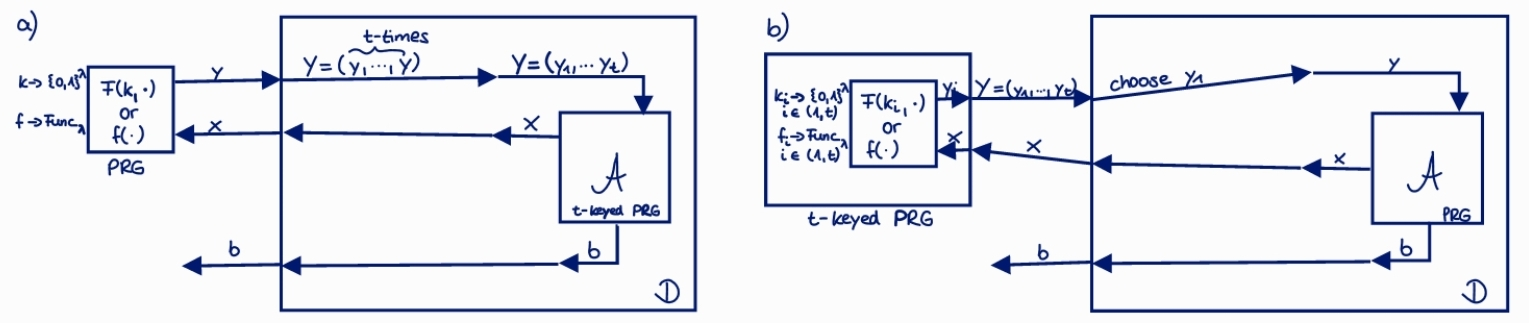
\includegraphics[width=\textwidth,height=\textheight,keepaspectratio]{ModKrypt_9-4.jpg}
    \centering
\end{figure}


